%%%%%%%%%%%%%%%%%%%%%%%%%%%%%%%%%%%%%%%%%%%%%%%%%%%%%%%%%%%%
%%  This Beamer template was created by Cameron Bracken.
%%  Anyone can freely use or modify it for any purpose
%%  without attribution.
%%
%%  Last Modified: January 9, 2009
%%

\documentclass[xcolor=x11names,compress]{beamer}


%% General document %%%%%%%%%%%%%%%%%%%%%%%%%%%%%%%%%%
\usepackage{graphicx}
\usepackage[spanish]{babel}
\usepackage{tikz}
\usepackage[latin1]{inputenc}  
\usepackage{listings}
\usepackage{hyperref}

%%%%%%%%%%%%%%%%%%%%%%%%%%%%%%%%%%%%%%%%%%%%%%%%%%%%%%


%% Beamer Layout %%%%%%%%%%%%%%%%%%%%%%%%%%%%%%%%%%
\beamertemplatenavigationsymbolsempty 
\useoutertheme[subsection=false,shadow]{miniframes}
\setbeamertemplate{footline}%{miniframes theme}
{%
	\begin{beamercolorbox}[colsep=1.0pt]{upper separation line foot}
	\end{beamercolorbox}
	\begin{beamercolorbox}[ht=0.25ex,dp=1.125ex,%
		leftskip=.3cm,rightskip=.3cm plus1fil]{author in head/foot}%
		\leavevmode{\usebeamerfont{author in head/foot}\insertshortauthor}%
		\hfill%
		{\usebeamerfont{institute in head/foot}\usebeamercolor[fg]{institute in head/foot}\insertshortinstitute}%
	\end{beamercolorbox}%
	\begin{beamercolorbox}[ht=4ex,dp=1.125ex,%
		leftskip=.3cm,rightskip=.3cm plus1fil]{title in head/foot}%
		{\usebeamerfont{title in head/foot}\insertshorttitle} \hfill     \Large{\insertframenumber}%
	\end{beamercolorbox}%
	\begin{beamercolorbox}[colsep=1.0pt]{lower separation line foot}
	\end{beamercolorbox}
}

\useinnertheme{default}
%\usefonttheme{serif}
\usepackage{helvet}

\setbeamerfont{title like}{shape=\scshape}
\setbeamerfont{frametitle}{shape=\scshape}

\definecolor{themeColor}{RGB}{102, 162, 102}
\definecolor{textColor}{RGB}{69, 69, 69}
\definecolor{backgroundColor}{RGB}{240,240,240}

\setbeamercolor*{lower separation line head}{bg=themeColor} 
\setbeamercolor*{normal text}{fg=textColor,bg=backgroundColor} 
\setbeamercolor*{alerted text}{fg=red} 
\setbeamercolor*{example text}{fg=black} 
\setbeamercolor*{structure}{fg=black} 

\setbeamercolor*{palette tertiary}{fg=black,bg=black!10} 
\setbeamercolor*{palette quaternary}{fg=black,bg=black!10} 

\lstset{ %
	backgroundcolor=\color{white},   % choose the background color; you must add \usepackage{color} or \usepackage{xcolor}
	basicstyle=\tiny,        % the size of the fonts that are used for the code
	breakatwhitespace=false,         % sets if automatic breaks should only happen at whitespace
	breaklines=true,                 % sets automatic line breaking
	captionpos=b,                    % sets the caption-position to bottom
	deletekeywords={...},            % if you want to delete keywords from the given language
	escapeinside={\%*}{*)},          % if you want to add LaTeX within your code
	extendedchars=true,              % lets you use non-ASCII characters; for 8-bits encodings only, does not work with UTF-8
	frame=single,                    % adds a frame around the code
	keepspaces=true,                 % keeps spaces in text, useful for keeping indentation of code (possibly needs columns=flexible)
	keywordstyle=\color{blue},       % keyword style
	language=Octave,                 % the language of the code
	morekeywords={*,...},            % if you want to add more keywords to the set
	numbers=left,                    % where to put the line-numbers; possible values are (none, left, right)
	numbersep=5pt,                   % how far the line-numbers are from the code
	rulecolor=\color{black},         % if not set, the frame-color may be changed on line-breaks within not-black text (e.g. comments (green here))
	showspaces=false,                % show spaces everywhere adding particular underscores; it overrides 'showstringspaces'
	showstringspaces=false,          % underline spaces within strings only
	showtabs=false,                  % show tabs within strings adding particular underscores
	stepnumber=2,                    % the step between two line-numbers. If it's 1, each line will be numbered
	tabsize=2,                       % sets default tabsize to 2 spaces
	title=\lstname                   % show the filename of files included with \lstinputlisting; also try caption instead of title
}

\renewcommand{\(}{\begin{columns}}
\renewcommand{\)}{\end{columns}}
\newcommand{\<}[1]{\begin{column}{#1}}
	\renewcommand{\>}{\end{column}}

\newcommand{\norm}[1]{\lVert#1\rVert}
%%%%%%%%%%%%%%%%%%%%%%%%%%%%%%%%%%%%%%%%%%%%%%%%%%

\setbeamertemplate{section page}
{
	\begin{centering}
		\vskip1em\par
		\begin{beamercolorbox}[sep=4pt,center]{part title}
			\usebeamerfont{section title}\insertsection\par
		\end{beamercolorbox}
	\end{centering}
}

\AtBeginSection[]
{
	\frame{\sectionpage}
	%\begin{frame}<beamer>
	%\frametitle{Outline}
	%\tableofcontents[
	% currentsection,
	%  sectionstyle=show/hide,
	%  subsectionstyle=show/show/hide
	%]
	%\end{frame}
}


\begin{document}
	
	
	%%%%%%%%%%%%%%%%%%%%%%%%%%%%%%%%%%%%%%%%%%%%%%%%%%%%%%
	%%%%%%%%%%%%%%%%%%%%%%%%%%%%%%%%%%%%%%%%%%%%%%%%%%%%%%
	{
		\setbeamercolor{background canvas}{bg=themeColor}
		\setbeamercolor{title}{bg=themeColor} 
		\begin{frame}
			\title{Inteligencia Artificial Aplicada\\ \textbf{Reconocimiento de im�genes}}
			\author{
				\textsc{	\footnotesize{Brayan Stiven Zapata Impat�}\\
						{\it brayan.inf @ gmail.com}\\\ \\}
			}
			\titlepage
		\end{frame}
	}
	
	%%%%%%%%%%%%%%%%%%%%%%%%%%%%%%%%%%%%%%%%%%%%%%%%%%%%%%
	%%%%%%%%%%%%%%%%%%%%%%%%%%%%%%%%%%%%%%%%%%%%%%%%%%%%%%
	
	\begin{frame}{�ndice}
		\tableofcontents[hideallsubsections]
	\end{frame}
	
	%%%%%%%%%%%%%%%%%%%%%%%%%%%%%%%%%%%%%%%%%%%%%%%%%%%%%%
	%%%%%%%%%%%%%%%%%%%%%%%%%%%%%%%%%%%%%%%%%%%%%%%%%%%%%%
	
	\section{\scshape Introducci�n}
	
	\begin{frame}
		\frametitle{Contexto}
		\begin{figure}[h]
			\centering
			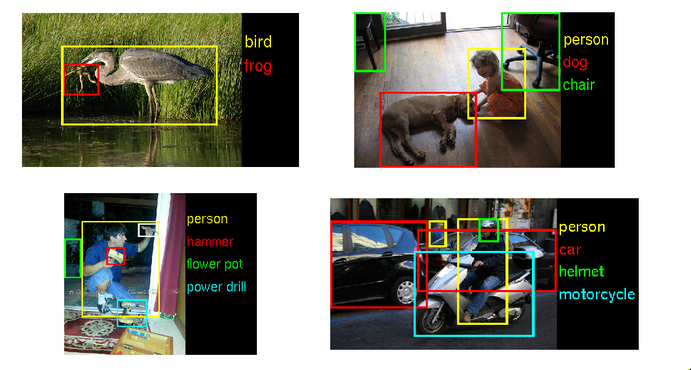
\includegraphics[width=1\textwidth]{img/introduccion}
			\caption{Ejemplo de reconocimiento de entidades en fotos.}
		\end{figure}
	\end{frame}
	
	%%%%%%%%%%%%%%%%%%%%%%%%%%%%%%%%%%%%%%%%%%%%%%%%%%%%%%
	%%%%%%%%%%%%%%%%%%%%%%%%%%%%%%%%%%%%%%%%%%%%%%%%%%%%%%
	
	\section{\scshape Metodolog�a}
	
	\begin{frame}
		\frametitle{Convolutional Neural Network}
		\begin{figure}[h]
			\centering
			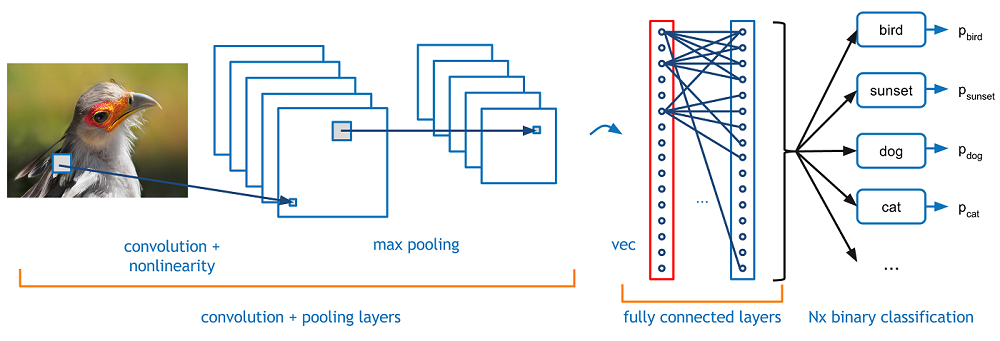
\includegraphics[width=1\textwidth]{img/cnn}
			\caption{Ejemplo de topolog�a de una red neuronal convolucional.}
		\end{figure}
	\end{frame}
	
	\begin{frame}
		\frametitle{Convolutional Neural Network}
		\begin{figure}[h]
			\centering
			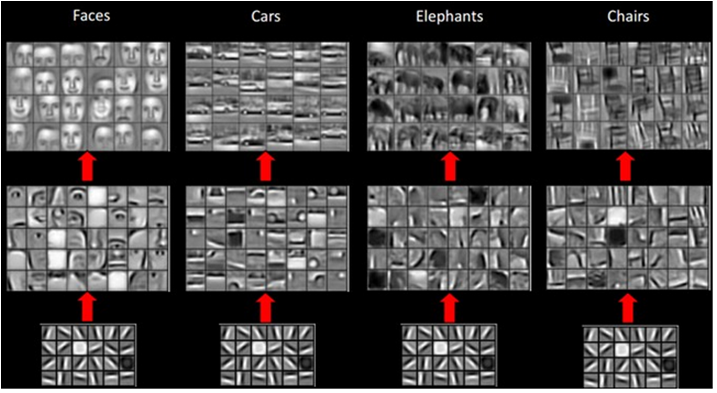
\includegraphics[width=1\textwidth]{img/cnnfeatures}
			\caption{Muestras de patrones aprendidos por las CNN.}
		\end{figure}
	\end{frame}
	
	\begin{frame}
		\frametitle{Tecnolog�as}
		\begin{figure}[h]
			\centering
			
\includegraphics[width=0.3\textwidth]{img/keras}
			
\includegraphics[width=0.57\textwidth]{img/tensorflow}
			
			\includegraphics[width=1\textwidth]{img/cnnarq}
			\caption{Principales librer�as utilizadas y topolog�a de CNN implementada.}
		\end{figure}
	\end{frame}
	
	
	%%%%%%%%%%%%%%%%%%%%%%%%%%%%%%%%%%%%%%%%%%%%%%%%%%%%%%
	%%%%%%%%%%%%%%%%%%%%%%%%%%%%%%%%%%%%%%%%%%%%%%%%%%%%%%
	
	\section{\scshape Experimentaci�n}
	
	\begin{frame}
		\frametitle{Configuraci�n}
	
		Entrenamiento utilizando 25.000 im�genes:
	
		\begin{itemize}
			\item 90\% reservado para entrenamiento de la red, restante para validaci�n
			
			\item 30 iteraciones
			
			\item Im�genes transformadas a 150 x 150 x 3
			
			\item 44.497.985 de par�metros o pesos a aprender por la topolog�a de la \textit{CNN}
			
			\item Ejecutado sobre GTX 960 4GB (1024 CUDA cores)
			
			\item Aproximadamente 75 minutos en ejecuci�n
			
			\item 86\% acierto sobre conjunto de validaci�n
		\end{itemize}
	\end{frame}	
	
	
	\begin{frame}
		\frametitle{Resultados}
		\begin{figure}[h]
			\centering
			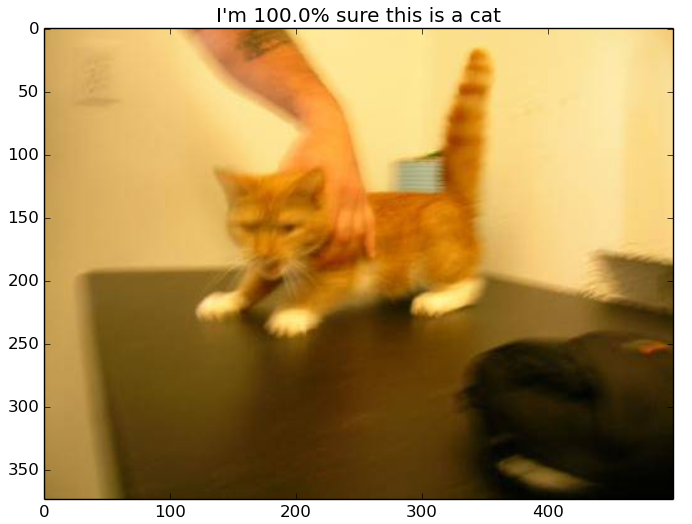
\includegraphics[width=0.55\textwidth]{img/gato-borroso}
			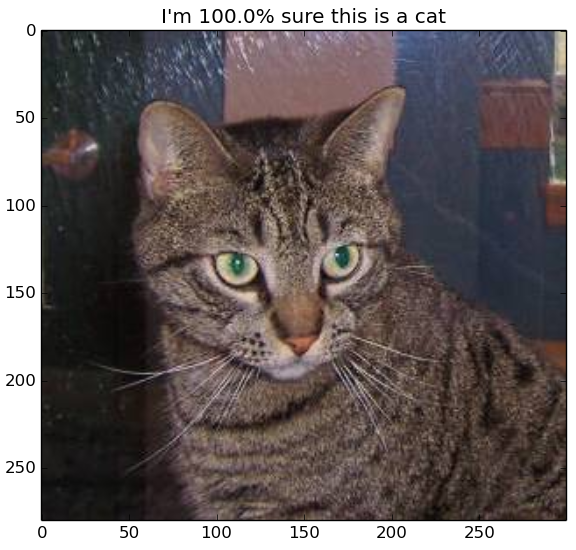
\includegraphics[width=0.45\textwidth]{img/cat1}
			\caption{Ejemplos de gatos bien etiquetados.}
		\end{figure}
	\end{frame}
	
	\begin{frame}
		\frametitle{Resultados}
		\begin{figure}[h]
			\centering
			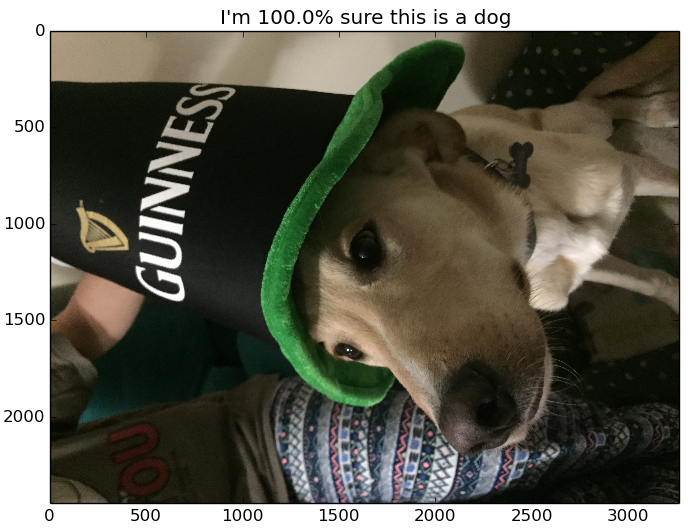
\includegraphics[width=0.6\textwidth]{img/guinness}
			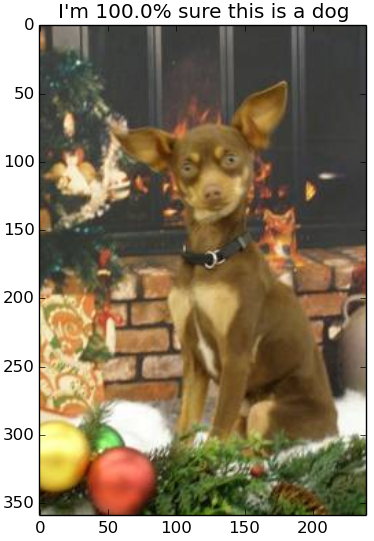
\includegraphics[width=0.32\textwidth]{img/dog1}
			\caption{Ejemplos de perros bien etiquetados.}
		\end{figure}
	\end{frame}
	
	
	\begin{frame}
		\frametitle{Resultados}
		\begin{figure}[h]
			\centering
			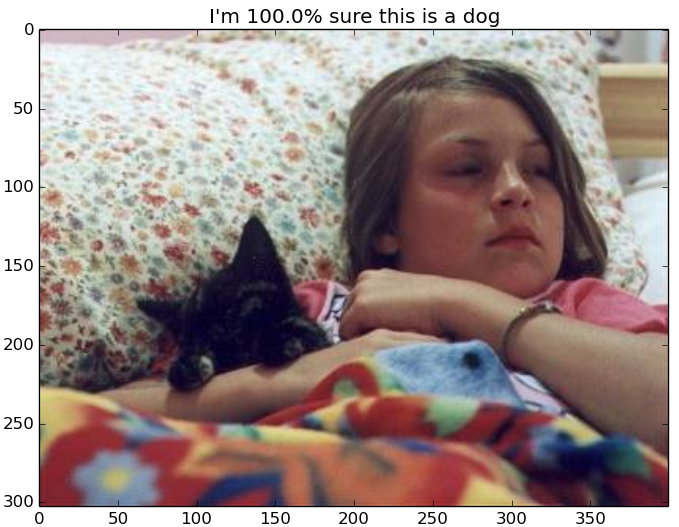
\includegraphics[width=0.49\textwidth]{img/gato-perro}
			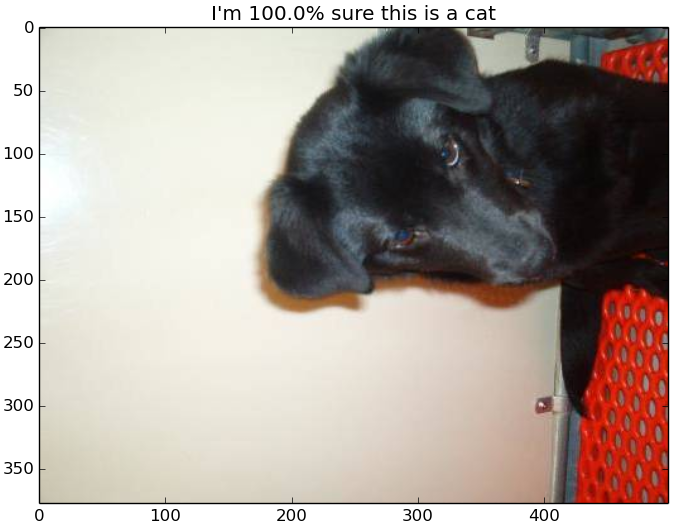
\includegraphics[width=0.49\textwidth]{img/perro-gato}
			\caption{Ejemplos de im�genes mal etiquetadas.}
		\end{figure}
	\end{frame}
	
	\begin{frame}
		\frametitle{Resultados}
		\begin{figure}[h]
			\centering
			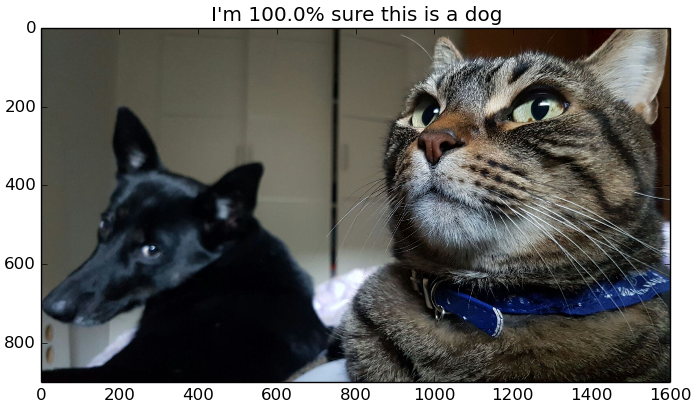
\includegraphics[width=1\textwidth]{img/ninatoy}
			\caption{Ejemplo cuando tenemos ambas clases en la misma imagen.}
		\end{figure}
	\end{frame}
	
	\begin{frame}
		\frametitle{Resultados}
		\begin{figure}[h]
			\centering
			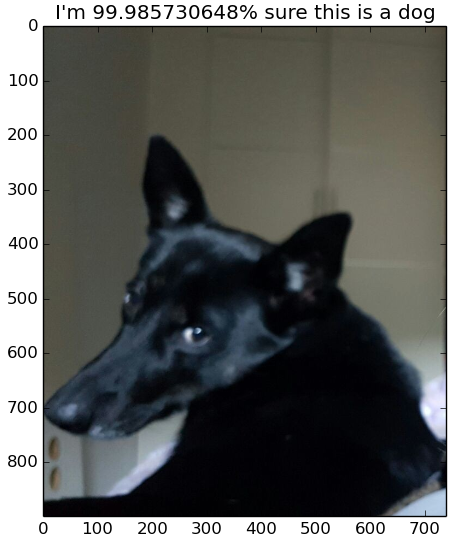
\includegraphics[width=0.45\textwidth]{img/nina}
			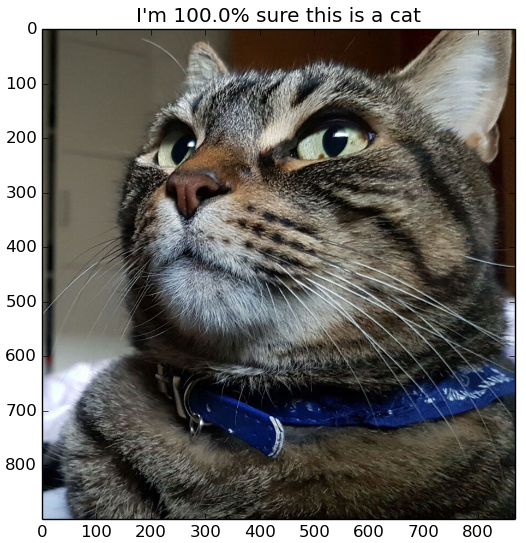
\includegraphics[width=0.45\textwidth]{img/toy}
			\caption{Etiquetado al dividir la imagen anterior.}
		\end{figure}
	\end{frame}

	%%%%%%%%%%%%%%%%%%%%%%%%%%%%%%%%%%%%%%%%%%%%%%%%%%%%%%
	%%%%%%%%%%%%%%%%%%%%%%%%%%%%%%%%%%%%%%%%%%%%%%%%%%%%%%	
	
	\section{\scshape Referencias}
	
	\begin{frame}[allowframebreaks]
	        \frametitle{Referencias}
	        \nocite{*}
	        \bibliographystyle{unsrt}
	        \bibliography{biblio}
	\end{frame}
	
	%%%%%%%%%%%%%%%%%%%%%%%%%%%%%%%%%%%%%%%%%%%%%%%%%%%%%%
	%%%%%%%%%%%%%%%%%%%%%%%%%%%%%%%%%%%%%%%%%%%%%%%%%%%%%%
	
	{
		\setbeamercolor{background canvas}{bg=themeColor}
		\setbeamercolor{title}{bg=themeColor} 
		\begin{frame}
			\title{Inteligencia Artificial Aplicada\\ \textbf{Reconocimiento de im�genes}}
			\author{
				\textsc{	\footnotesize{Brayan Stiven Zapata Impat�}\\
					{\it brayan.inf @ gmail.com }\\\ \\}
			}
			\date{
				\vspace{1cm}
				\normalsize{GRACIAS POR SU ATENCI�N}
			}
			\titlepage
		\end{frame}
	}
	
	
\end{document}